 Il seguente listato valuta la spline naturale e quella not-a-knot per le funzioni date:
\lstinputlisting[language=Matlab]{cap_4/es5/es5.m}

\begin{figure}
\centering
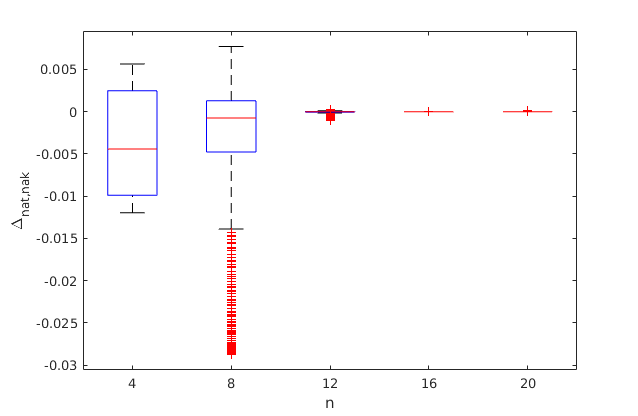
\includegraphics[scale=0.7]{cap_4/es5/errors}
\caption{$\Delta_{nat, nak}$ per la funzione di Runge}
\label{err_runge}
\end{figure}
\begin{figure}
\centering
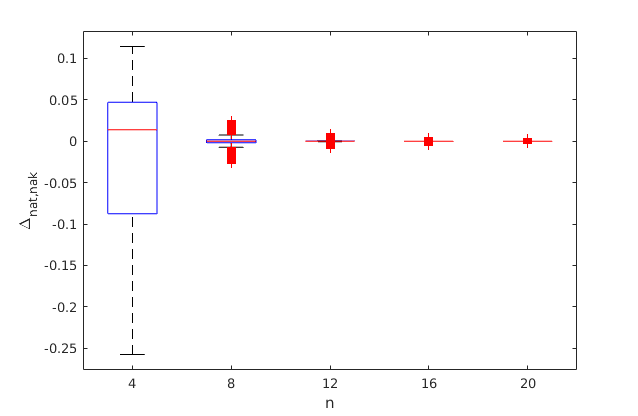
\includegraphics[scale=0.5]{cap_4/es5/errors_sin}
\caption{$\Delta_{nat, nak}$ per la funzione sin(x)*x}
\label{err_sin}
\end{figure}
Nelle figure \ref{err_runge} e \ref{err_sin} possiamo vedere come l'errore nel tra una spline naturale e una spline not a knot sia visibilmente inferiore nel caso della funziona Sin(x)*x.

Nei seguenti grafici invece vediamo l'approssimazione delle spline naturali e not a knot per le medesime funzioni, comparate con il grafico della funzione originale.

\begin{figure}
\centering
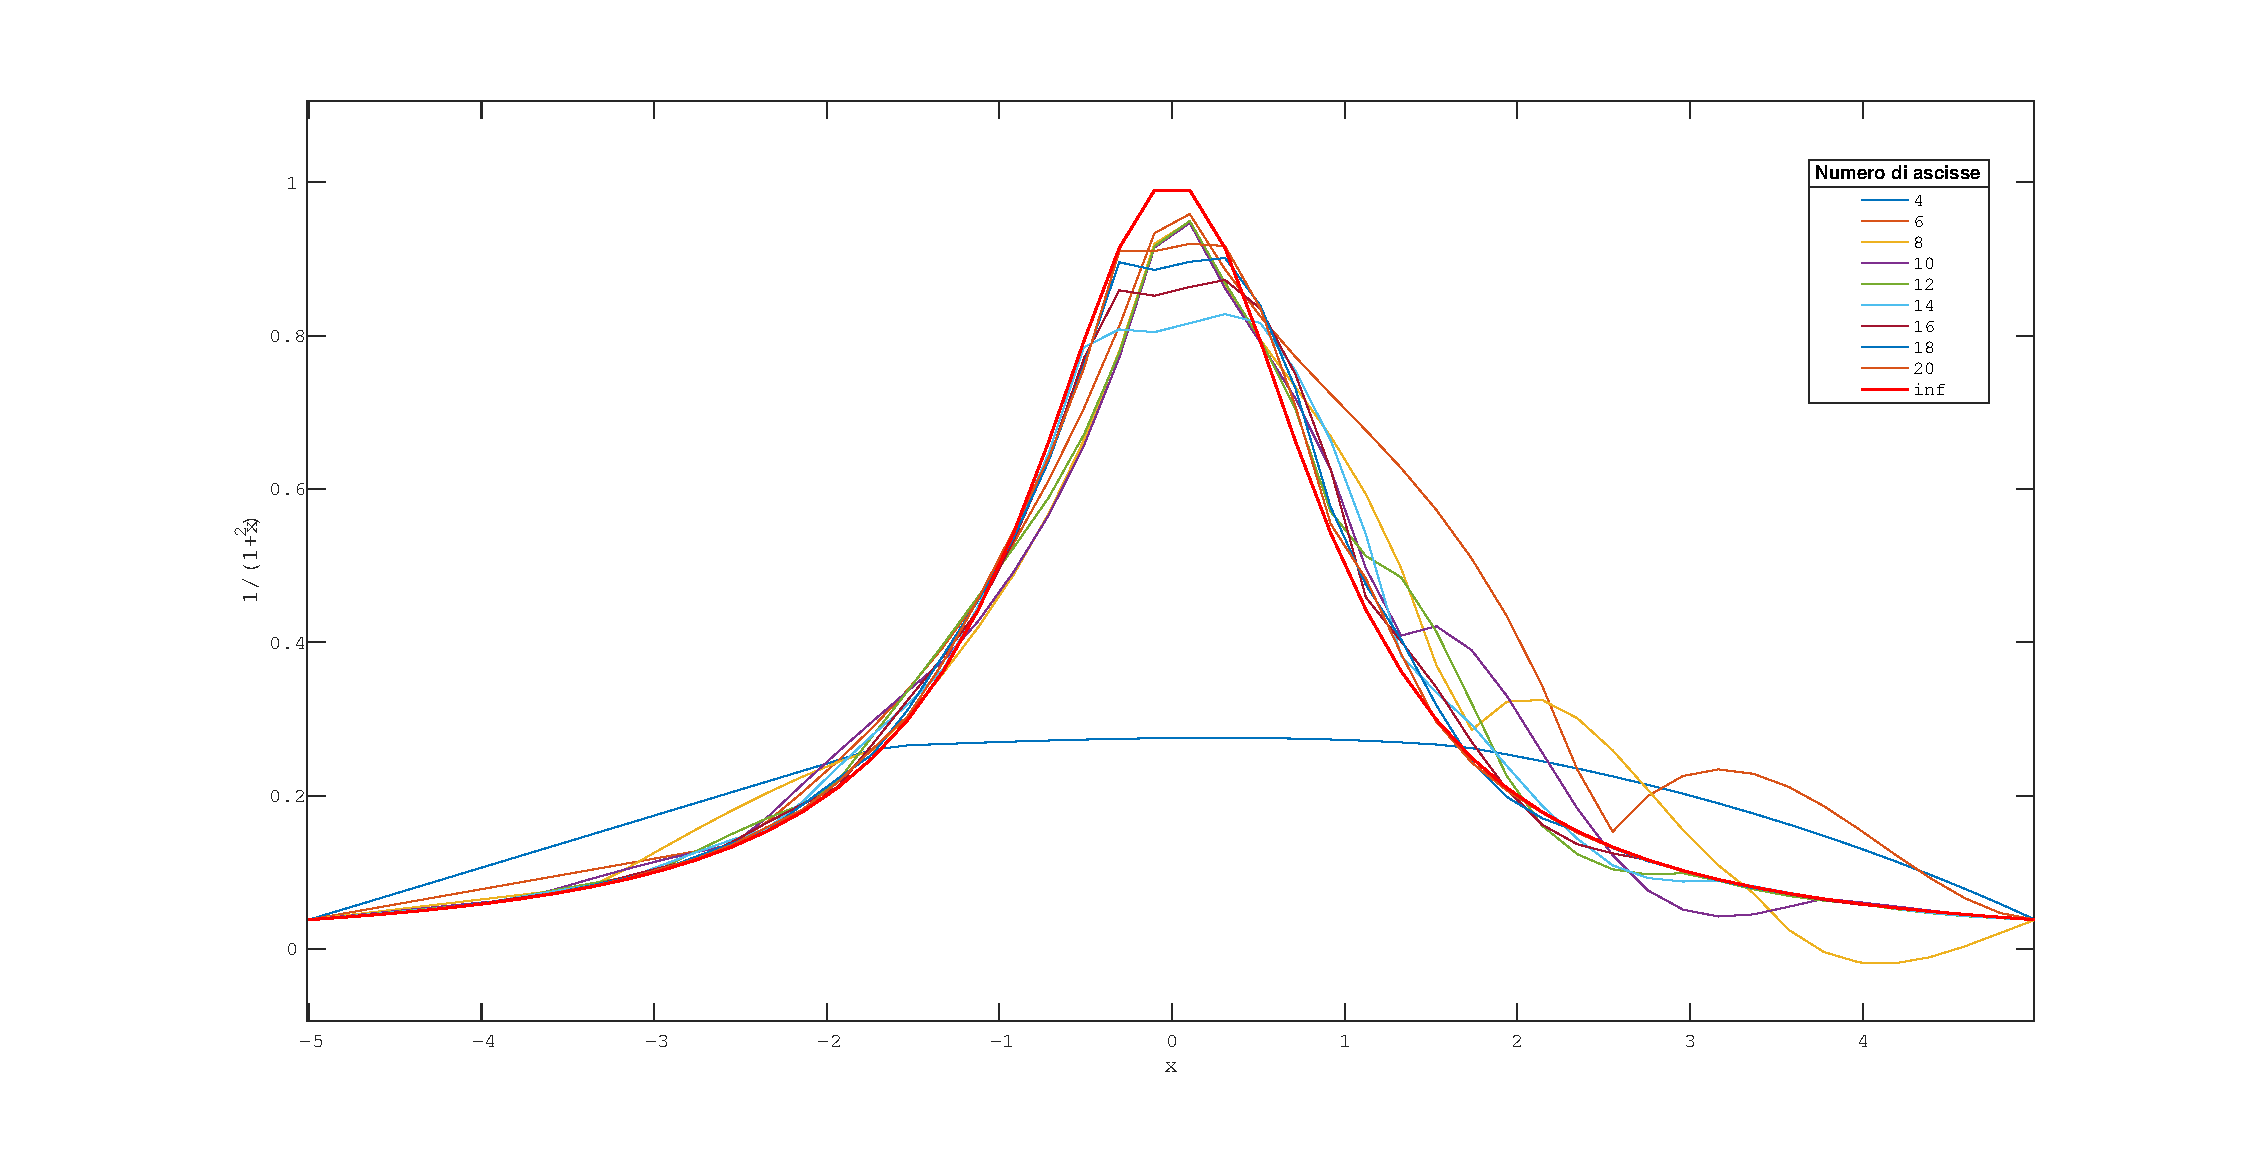
\includegraphics[scale=0.5]{cap_4/es5/runge_nat}
\caption{$\frac{1}{1+x^2}$ interpolata con spline naturale}
\label{plot_runge_nat}
\end{figure}


\begin{figure}
\centering
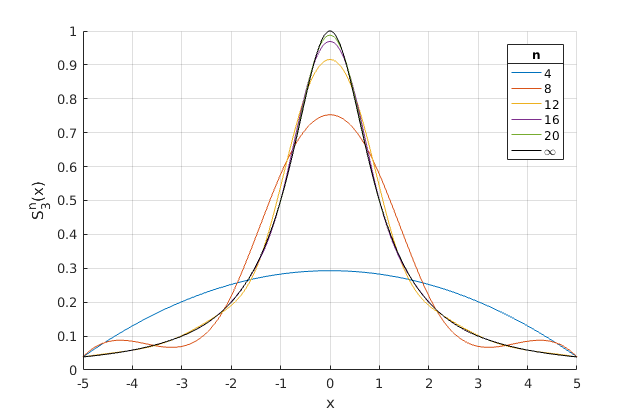
\includegraphics[scale=0.43]{cap_4/es5/runge_nak}
\caption{$\frac{1}{1+x^2}$ interpolata con spline not-a-knot}
\label{plot_runge_nak}
\end{figure}

\begin{figure}
\centering
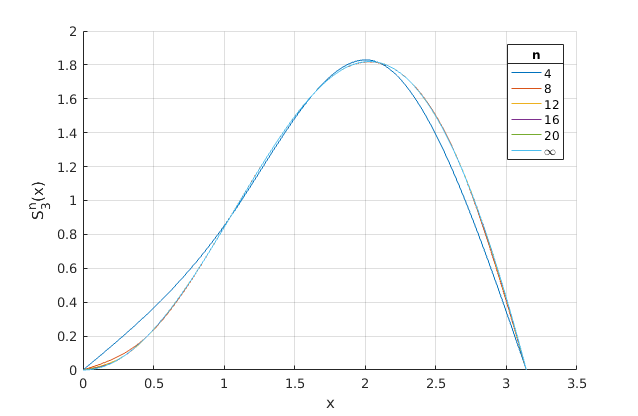
\includegraphics[scale=0.5]{cap_4/es5/sin_nat}
\caption{$x*sin(x)$ interpolata con spline naturale}
\label{plot_sin_nat}
\end{figure}


\begin{figure}
\centering
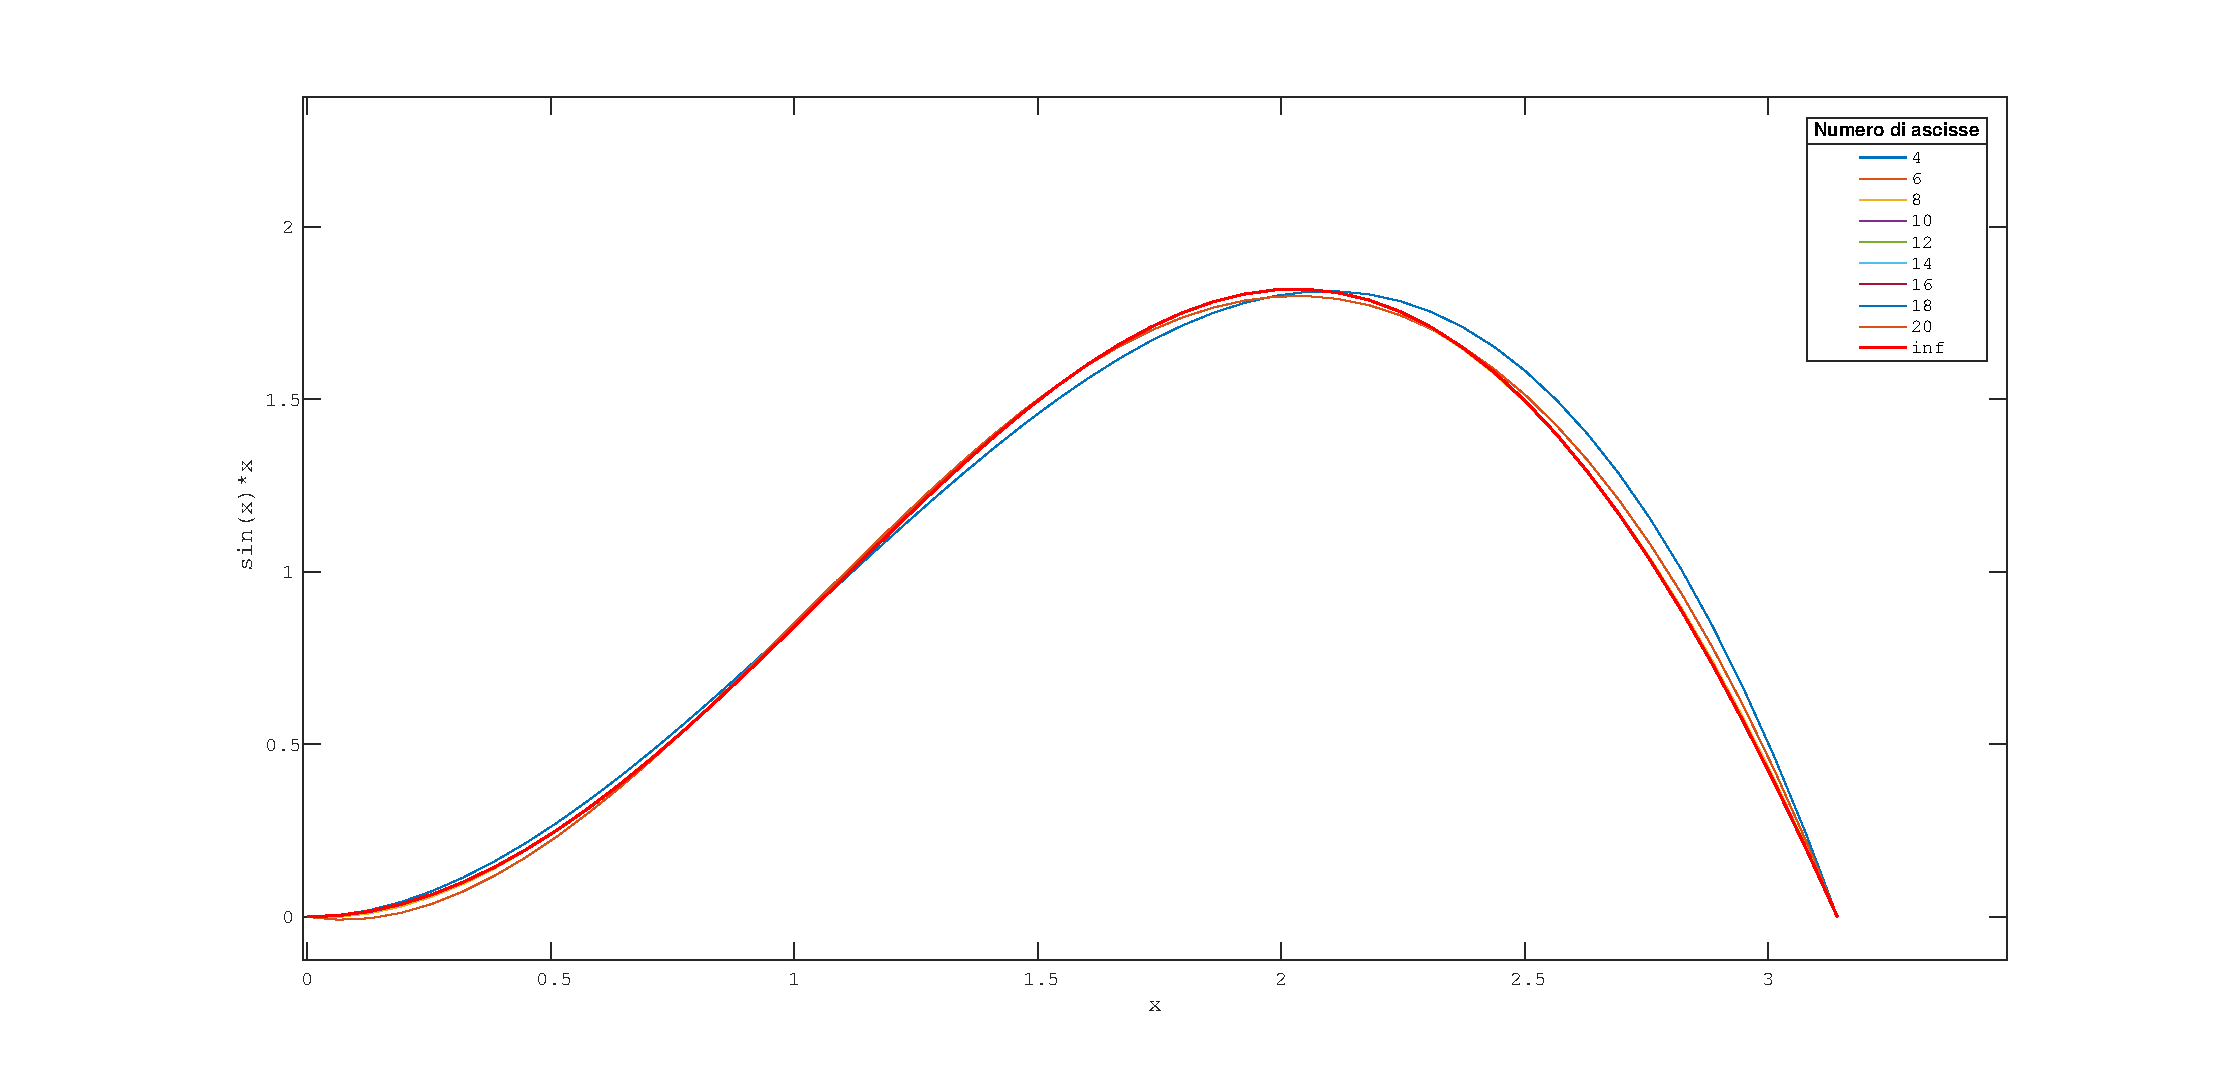
\includegraphics[scale=0.43]{cap_4/es5/sin_nak}
\caption{$x*sin(x)$ interpolata con spline not-a-knot}
\label{plot_sin_nak}
\end{figure}
